\documentclass[svgnames]{standalone}

\usepackage[utf8]{inputenc}
\usepackage{tikz}
\usetikzlibrary{mindmap}

\begin{document}

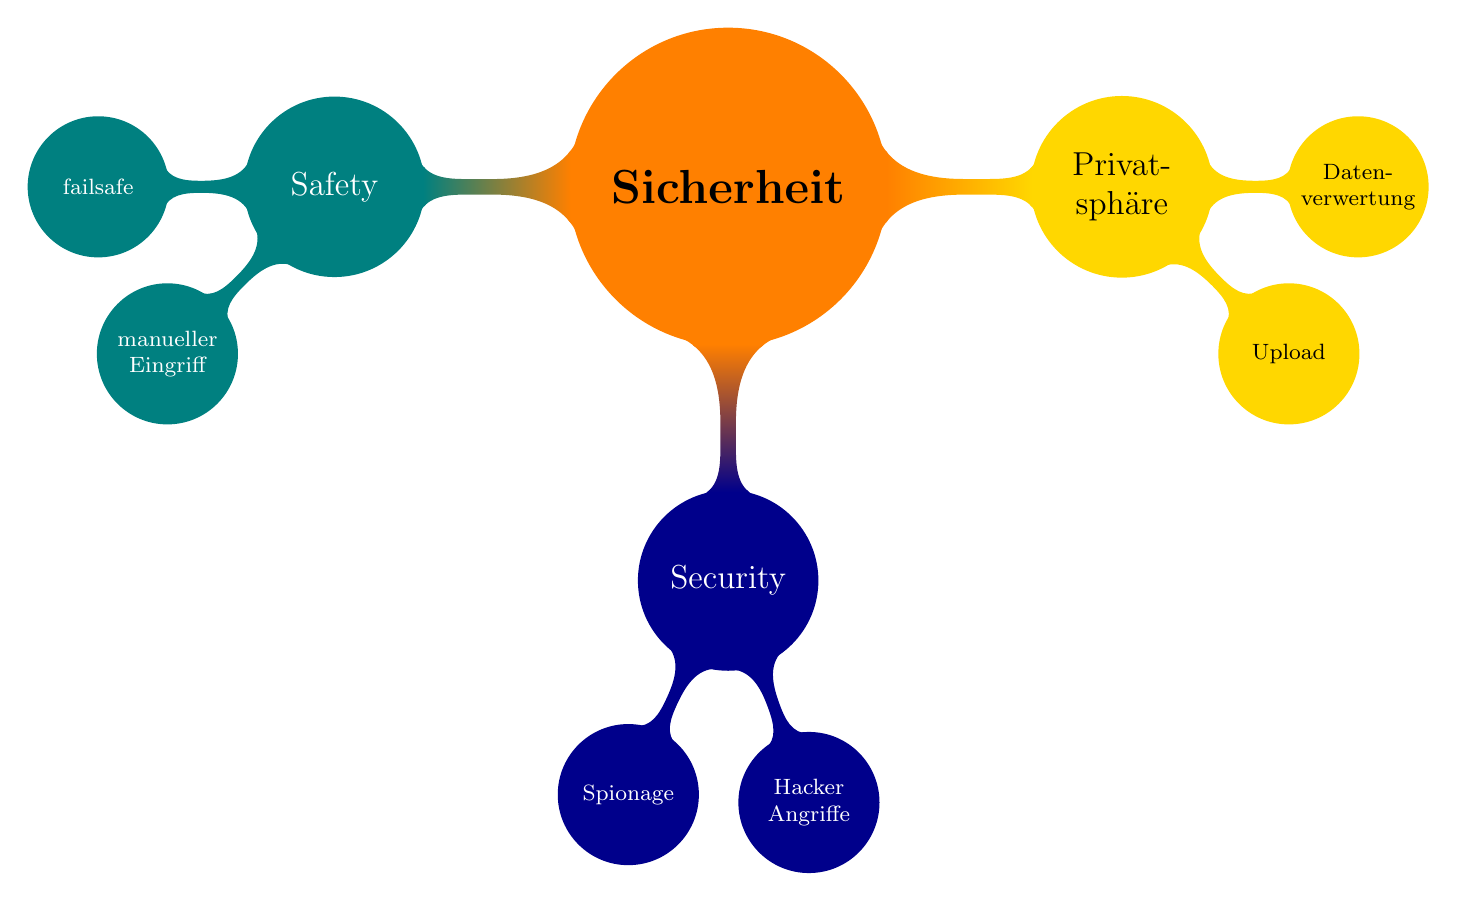
\begin{tikzpicture}[mindmap, grow cyclic, every node/.style=concept, concept color=orange,
    level 1/.append style={level distance=5cm,sibling angle=90,font=\large},
    level 2/.append style={level distance=3cm,sibling angle=45}]

  \node{\textbf{\LARGE{Sicherheit}}} [clockwise from=0]
  child [concept color=Gold] { node {Privat\-sphäre} [clockwise from=0]
      child { node {Daten\-verwertung}}
      child { node {Upload}}
    }
  child [concept color=DarkBlue,text=white] { node {Security} [clockwise from=290]
      child { node {Hacker Angriffe}}
      child { node {Spionage}}
    }
  child [concept color=teal,text=white] { node {Safety} [counterclockwise from=180]
      child { node {failsafe}}
      child { node {manueller Eingriff}}
    };
\end{tikzpicture}

\end{document}
